\documentclass[tikz]{standalone}
\usetikzlibrary{calc,trees,positioning,arrows,chains,shapes.geometric,%
    decorations.pathreplacing,decorations.pathmorphing,shapes,%
    matrix,shapes.symbols,fit}
\usepackage{ifthen}
\pgfdeclarelayer{back}
\pgfsetlayers{back,main}


\makeatletter
\tikzset{
  fitting node/.style={
    inner sep=0pt,
    fill=none,
    draw=none,
    reset transform,
    fit={(\pgf@pathminx,\pgf@pathminy) (\pgf@pathmaxx,\pgf@pathmaxy)}
  },
  reset transform/.code={\pgftransformreset}
}
\makeatother

\pgfmathdeclarerandomlist{MyRandomColors}{%
    {red}%
    {magenta}%
    {olive}%
    {brown}%
    {violet}%
    {gray}%
    {purple}%
    {yellow}%
    {orange}%
    {cyan}%
    {green}%    
}

% \pgfmathdeclarerandomlist{MyRandomColors}{%
%     {red}%
%     {red!25}%
%     {magenta}%
%     {magenta!25}%
%     {olive}%
%     {olive!25}%
%     {brown}%
%     {brown!10}%
%     {violet}%
%     {violet!25}%
%     {gray}%
%     {purple}%
%     {yellow}%
%     {orange}%
%     {orange!25}%
%     {cyan}%
%     {green}%    
% }%

\begin{document}
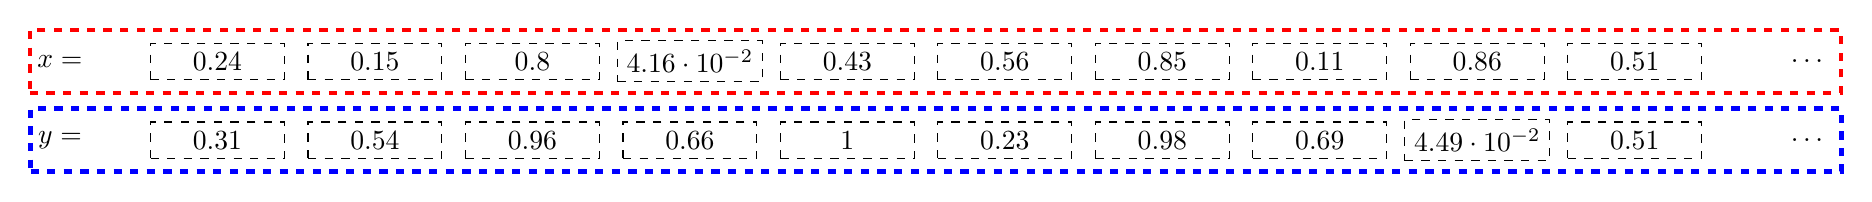
\begin{tikzpicture}


  \node at(-2,1) (x_pos) {$x =$};
  \node at(-2,0.5) (center) {};
  \node at(-2,0) (y_pos) {$y =$};

  \pgfmathsetseed{2017}

  \foreach \n in {1,...,10}{
    
    \pgfmathsetmacro{\xcoor}{rnd}% x-coordinate
    \pgfmathsetmacro{\ycoor}{rnd}% y-coordinate

    \node [draw,rectangle,dashed,minimum width=1.7cm] at($(x_pos)+(\n*2cm,0)$) (x_num_\n) {$\pgfmathprintnumber[precision=2]{\xcoor}$};
    \node [draw,rectangle,dashed,minimum width=1.7cm] at($(y_pos)+(\n*2cm,0)$) (y_num_\n) {$\pgfmathprintnumber[precision=2]{\ycoor}$};
;
  }

  \node [draw,ultra thick,color=red ,rectangle,dashed,minimum width=23cm,minimum height=.8cm,anchor=west] at($(x_pos.west)$) () {};
  \node [draw,ultra thick,color=blue,rectangle,dashed,minimum width=23cm,minimum height=.8cm,anchor=west] at($(y_pos.west)$) () {};

  \node [right=of x_num_10] () {\dots};
  \node [right=of y_num_10] () {\dots};
\end{tikzpicture}
\end{document}
